\chapter{Implementacija i korisničko sučelje}
		
		
		\section{Korištene tehnologije i alati}
		
			\textbf{\textit{dio 2. revizije}}
			
			 \textit{Detaljno navesti sve tehnologije i alate koji su primijenjeni pri izradi dokumentacije i aplikacije. Ukratko ih opisati, te navesti njihovo značenje i mjesto primjene. Za svaki navedeni alat i tehnologiju je potrebno \textbf{navesti internet poveznicu} gdje se mogu preuzeti ili više saznati o njima}.
			
			
			\eject 
		
	
		\section{Ispitivanje programskog rješenja}
			
			\textbf{\textit{dio 2. revizije}}\\
			
			 
			
			\subsection{Ispitivanje komponenti}
			     Sastavne programske komponente formirane su od nekoliko jedinica, uključujući osnovne dijelove programa poput razreda, pripadajućih metoda i atributa, koje međusobno intenzivno surađuju. Interakcija se ostvaruje kroz proceduralna sučelja, gdje svaka komponenta enkapsulira određeni skup funkcionalnosti koje druge komponente mogu pozivati. Evaluacija komponenata izvodi se s pomoću Junit radnog okvira, koji automatizira proces testiranja. Upotrebom dviju vrsta testova, jednih u uobičajenim uvjetima rada i drugih s unosom neispravnih i rubnih uvjeta, analizira se očekivano ponašanje razreda i unaprijed definirani izlaz metoda.
            Za testiranje BookService metoda koristili smo sučelja Knjiga, Pondua, i BookRepository. Prvo smo testirali saveBook metodu.
           \begin{lstlisting}[language=Java, label=lst:java_example, basicstyle=\scriptsize, baselinestretch=0.9]
 @Test
    @DisplayName("Testiranje saveBook metode")
    void testSaveBook() {
        // Priprema podataka
        Knjiga knjiga = new Knjiga();
        List<Ponuda> ponude = new ArrayList<>();
        knjiga.setNaziv("Naslov knjige");
        knjiga.setIsbn("100");
        knjiga.setAutor("autor");
        knjiga.setIzdavac("izdavac");
        knjiga.setBrojIzdanja(1);
        knjiga.setOpis("opis");
        knjiga.setGodIzdanja(2005);
        knjiga.setSlikaURL("url");
        knjiga.setId(1L);
        knjiga.setOznaka("oznaka");
        knjiga.setKategorija("kategorija");
        knjiga.setStanjeOcuvanosti("st_oc");
        knjiga.setZahtjevi(50);
        knjiga.setZanr("zanr");
        knjiga.setPonude(ponude);


        when(bookRepository.save(any(Knjiga.class))).thenReturn(knjiga);


        Knjiga savedKnjiga = bookService.saveBook(knjiga);


        verify(bookRepository, times(1)).save(knjiga);
        assertNotNull(savedKnjiga);
        assertEquals("Naslov knjige", savedKnjiga.getNaziv());
        assertEquals("100", savedKnjiga.getIsbn());
        assertEquals("autor", savedKnjiga.getAutor());
        assertEquals("izdavac", savedKnjiga.getIzdavac());
        assertEquals(1, savedKnjiga.getBrojIzdanja());
        assertEquals("opis", savedKnjiga.getOpis());
        assertEquals(2005, savedKnjiga.getGodIzdanja());
        assertEquals("url", savedKnjiga.getSlikaURL());
        assertEquals(1L, savedKnjiga.getId());
        assertEquals("oznaka", savedKnjiga.getOznaka());
        assertEquals("kategorija", savedKnjiga.getKategorija());
        assertEquals("st_oc", savedKnjiga.getStanjeOcuvanosti());
        assertEquals(50, savedKnjiga.getZahtjevi());
        assertEquals("zanr", savedKnjiga.getZanr());
        assertNotNull(savedKnjiga.getPonude());

    }
\end{lstlisting}

   
			A zatim smo testirali deleteBook metodu. 
                  \begin{lstlisting}[language=Java, label=lst:java_example, basicstyle=\scriptsize, baselinestretch=0.9]
 @Test
    @DisplayName("Testiranje deleteBook metode.")
    void testDeleteBook(){
        Long bookIdToDelete = 1L;
        bookService.deleteBook(bookIdToDelete);
        verify(bookRepository).deleteById(bookIdToDelete);
    }
    
\end{lstlisting}

            Zatim smo testirali KorisnikService. Za to smo koristili sučelja Korisnik, Ponuda, i KorisnikRepository.
            
			Prvo smo testirali dohvaćanje korisnika. 
                  \begin{lstlisting}[language=Java, label=lst:java_example, basicstyle=\scriptsize, baselinestretch=0.9]
 @Test
    @DisplayName("Test dohvaćanja korisnika.")
    void testGetUserById() {
        Long userId = 1L;
        Korisnik mockKorisnik = new Korisnik();
        List<Ponuda> ponude = new ArrayList<>();

        mockKorisnik.setId(userId);
        mockKorisnik.setUsername("username");
        mockKorisnik.setPassword("password");
        mockKorisnik.setEmail("email@gmail.com");
        mockKorisnik.setOdobren(false);
        mockKorisnik.setTip("tip");
        mockKorisnik.setAdresa("adresa");
        mockKorisnik.setTelefon("123456789");
        mockKorisnik.setPonude(ponude);
        mockKorisnik.setPrijavljen(false);
        mockKorisnik.setURLL("url");
        mockKorisnik.setNaziv("naziv");

        when(korisnikRepository.findById(userId)).thenReturn(Optional.of(mockKorisnik));

        Korisnik result = korisnikService.getUserById(userId);

        assertEquals(userId, result.getId());
        assertEquals("adresa", result.getAdresa());
        assertEquals("123456789", result.getTelefon());
        assertEquals("tip", result.getTip());
        assertEquals("email@gmail.com", result.getEmail());
        assertEquals("password", result.getPassword());
        assertEquals("username", result.getUsername());
        assertEquals(false, result.getOdobren());
        assertNotNull(ponude);
        assertEquals(false, result.isPrijavljen());
        assertEquals("url", result.getURLL());
        assertEquals("naziv", result.getNaziv());
    }

    
\end{lstlisting}
            
			Zatim smo testirali funkcionalnost spremanja korisnika. 
                  \begin{lstlisting}[language=Java, label=lst:java_example, basicstyle=\scriptsize, baselinestretch=0.9]
 @Test
    @DisplayName("Test spremanja korisnika.")
    void saveUserTest(){
        Long userId = 1L;
        Korisnik mockKorisnik = new Korisnik();
        List<Ponuda> ponude = new ArrayList<>();

        mockKorisnik.setId(userId);
        mockKorisnik.setUsername("username");
        mockKorisnik.setPassword("password");
        mockKorisnik.setEmail("email@gmail.com");
        mockKorisnik.setOdobren(false);
        mockKorisnik.setTip("tip");
        mockKorisnik.setAdresa("adresa");
        mockKorisnik.setTelefon("123456789");
        mockKorisnik.setPonude(ponude);
        mockKorisnik.setPrijavljen(false);
        mockKorisnik.setURLL("url");
        mockKorisnik.setNaziv("naziv");


        when(korisnikRepository.save(any(Korisnik.class))).thenReturn(mockKorisnik);

        Korisnik savedKorisnik = korisnikService.saveKorisnik(mockKorisnik);

        verify(korisnikRepository, times(1)).save(mockKorisnik);
        
        assertEquals(userId, savedKorisnik.getId());
        assertEquals("adresa", savedKorisnik.getAdresa());
        assertEquals("123456789", savedKorisnik.getTelefon());
        assertEquals("tip", savedKorisnik.getTip());
        assertEquals("email@gmail.com", savedKorisnik.getEmail());
        assertEquals("password", savedKorisnik.getPassword());
        assertEquals("username", savedKorisnik.getUsername());
        assertEquals(false, savedKorisnik.getOdobren());
        assertNotNull(ponude);
        assertEquals(false, savedKorisnik.isPrijavljen());
        assertEquals("url", savedKorisnik.getURLL());
        assertEquals("naziv", savedKorisnik.getNaziv());
    }
    
\end{lstlisting}
            
			Nakon toga smo testirali ponudu, to jest OfferService. Za te testove smo koristili sučelja Knjiga, Korisnik, Ponuda, PonudaDto, BookRepository, KorisnikRepository, OfferRepository i OfferService. 
            Prvo smo testirali brisanje ponude. 
            
                  \begin{lstlisting}[language=Java, label=lst:java_example, basicstyle=\scriptsize, baselinestretch=0.9]
 @Test
    @DisplayName("Testiranje brisanja ponude.")
    void deleteOfferTest() {
        Long offerId = 1L;

        offerService.deleteOffer(offerId);

        verify(offerRepository, times(1)).deleteById(offerId);
    }
    
\end{lstlisting}
            A zatim smo testirali spremanje ponude. 
                  \begin{lstlisting}[language=Java, label=lst:java_example, basicstyle=\scriptsize, baselinestretch=0.9]
  @Test
    @DisplayName("Testiranje spremanja ponude.")
    void saveOffer() {
        // Arrange
        PonudaDto ponudaDto = new PonudaDto();
        ponudaDto.setPonuditeljId(1L);
        ponudaDto.setKnjigaId(2L);
        ponudaDto.setCijena(100);
        ponudaDto.setBrojPrimjeraka(5);

        Korisnik mockKorisnik = new Korisnik();
        Knjiga mockKnjiga = new Knjiga();
        Ponuda mockPonuda = new Ponuda();

        when(korisnikRepository.findById(ponudaDto.getPonuditeljId())).thenReturn(java.util.Optional.of(mockKorisnik));
        when(bookRepository.findById(ponudaDto.getKnjigaId())).thenReturn(java.util.Optional.of(mockKnjiga));
        when(offerRepository.save(any(Ponuda.class))).thenReturn(mockPonuda);


        Ponuda resultPonuda = offerService.saveOffer(ponudaDto);

        verify(offerRepository).save(any(Ponuda.class));

        assertEquals(mockPonuda, resultPonuda);
    }

    
\end{lstlisting}
            Zatim smo testirali kada spremamo ponudu, a ne postoji taj userId.
                  \begin{lstlisting}[language=Java, label=lst:java_example, basicstyle=\scriptsize, baselinestretch=0.9]
 @Test
    @DisplayName("Testiranje kada spremamo ponudu. a ne postoji taj userId.")
    void saveOfferInvalid() {
        PonudaDto ponudaDto = new PonudaDto();
        ponudaDto.setPonuditeljId(1L);
        ponudaDto.setKnjigaId(2L);
        ponudaDto.setCijena(100);
        ponudaDto.setBrojPrimjeraka(5);

        when(korisnikRepository.findById(ponudaDto.getPonuditeljId())).thenReturn(Optional.empty());

        // Act & Assert
        // Verify that ResponseStatusException is thrown with the correct status and message
        ResponseStatusException exception = Assertions.assertThrows(ResponseStatusException.class, () -> {
            offerService.saveOffer(ponudaDto);
        });

        assertEquals(HttpStatus.NOT_FOUND, exception.getStatusCode());
        assertEquals("Korisnik not found", exception.getReason());
    }
    
\end{lstlisting}

            Svi testovi su se ispravno izveli s očekivanim rezultatima. 
            \eject
			
			
			\begin{figure}[H]
				\includegraphics[width=\textwidth]{slike/UnitiTest1.PNG} %veličina u odnosu na širinu linije
				\centering
				\caption{Rezultat testiranja BookService }
				\label{fig:BookService1}
			\end{figure}
			
			\eject
            \eject
			
			
			\begin{figure}[H]
				\includegraphics[width=\textwidth]{slike/UnitiTest3.PNG} %veličina u odnosu na širinu linije
				\centering
				\caption{Rezultat testiranja KorisnikService }
				\label{fig:KorisnikService1}
			\end{figure}
			
			\eject
            \eject
			
			
			\begin{figure}[H]
				\includegraphics[width=\textwidth]{slike/UnitiTest2.PNG} %veličina u odnosu na širinu linije
				\centering
				\caption{Rezultat testiranja OfferService}
				\label{fig:OfferService1}
			\end{figure}
			
			\eject
			
			
			
			
			
			\subsection{Ispitivanje sustava}
			
			 \textit{Potrebno je provesti i opisati ispitivanje sustava koristeći radni okvir Selenium\footnote{\url{https://www.seleniumhq.org/}}. Razraditi \textbf{minimalno 4 ispitna slučaja} u kojima će se ispitati redovni slučajevi, rubni uvjeti te poziv funkcionalnosti koja nije implementirana/izaziva pogrešku kako bi se vidjelo na koji način sustav reagira kada nešto nije u potpunosti ostvareno. Ispitni slučaj se treba sastojati od ulaza (npr. korisničko ime i lozinka), očekivanog izlaza ili rezultata, koraka ispitivanja i dobivenog izlaza ili rezultata.\\ }
			 
			 \textit{Izradu ispitnih slučajeva pomoću radnog okvira Selenium moguće je provesti pomoću jednog od sljedeća dva alata:}
			 \begin{itemize}
			 	\item \textit{dodatak za preglednik \textbf{Selenium IDE} - snimanje korisnikovih akcija radi automatskog ponavljanja ispita	}
			 	\item \textit{\textbf{Selenium WebDriver} - podrška za pisanje ispita u jezicima Java, C\#, PHP koristeći posebno programsko sučelje.}
			 \end{itemize}
		 	\textit{Detalji o korištenju alata Selenium bit će prikazani na posebnom predavanju tijekom semestra.}
			
			\eject 
		
		
		\section{Dijagram razmještaja}
			
			Dijagrami razmještaja prikazuju fizičku arhitekturu i topologiju programskog sustava te programsku potporu koja se koristi u njegovom radnom okruženju. Na korisničkom računalu se nalazi web preglednik koji služi za pristupanje web aplikaciji. Na poslužiteljskom računalu se nalaze web poslužitelj i poslužitelj baze podataka koji međusobno komuniciraju. Sustav koristi arhitekturu "klijent - poslužitelj", a komunikacija između korisnika(klijent, izdavač, administrator) i poslužitelja se odvija preko HTTP protokola.
			
			\begin{figure}[H]
				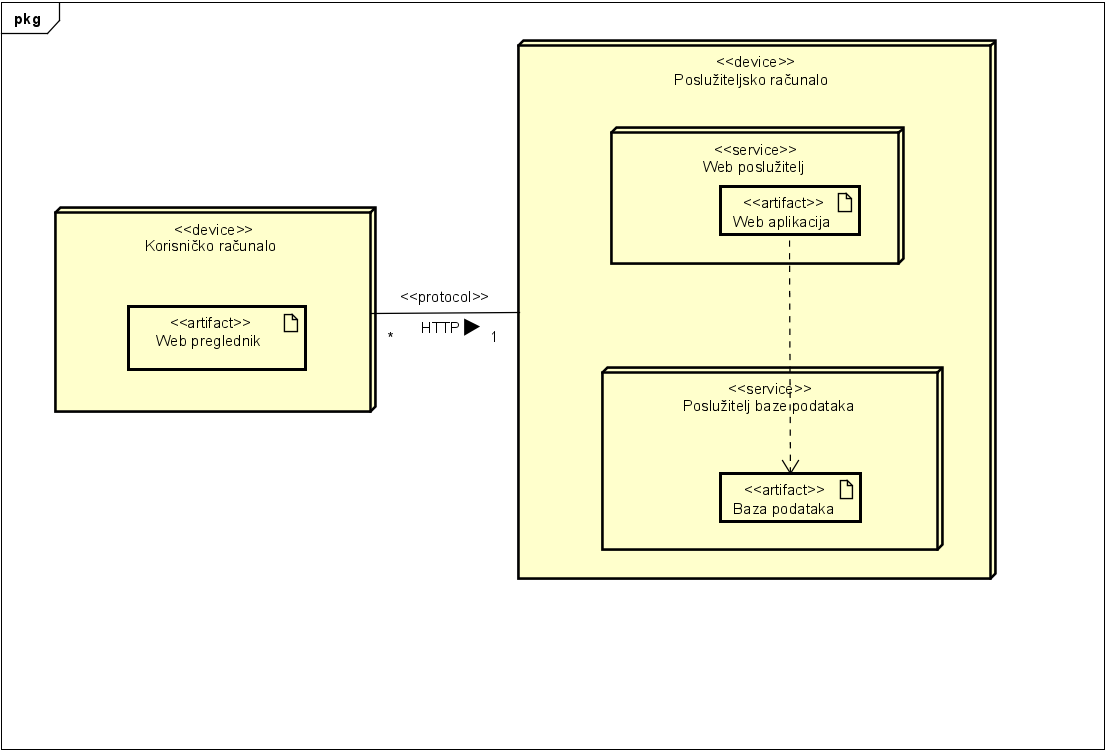
\includegraphics[width=\textwidth]{dijagrami/DijagramRazmjestaja.PNG} %veličina u odnosu na širinu linije
				\centering
				\caption{Dijagram razmještaja}
				\label{fig:diagrazmjestaja}
			\end{figure}
			
			
			\eject 
		
		\section{Upute za puštanje u pogon}
		
			\textbf{\textit{dio 2. revizije}}\\
		
			 \textit{U ovom poglavlju potrebno je dati upute za puštanje u pogon (engl. deployment) ostvarene aplikacije. Na primjer, za web aplikacije, opisati postupak kojim se od izvornog kôda dolazi do potpuno postavljene baze podataka i poslužitelja koji odgovara na upite korisnika. Za mobilnu aplikaciju, postupak kojim se aplikacija izgradi, te postavi na neku od trgovina. Za stolnu (engl. desktop) aplikaciju, postupak kojim se aplikacija instalira na računalo. Ukoliko mobilne i stolne aplikacije komuniciraju s poslužiteljem i/ili bazom podataka, opisati i postupak njihovog postavljanja. Pri izradi uputa preporučuje se \textbf{naglasiti korake instalacije uporabom natuknica} te koristiti što je više moguće \textbf{slike ekrana} (engl. screenshots) kako bi upute bile jasne i jednostavne za slijediti.}
			
			
			 \textit{Dovršenu aplikaciju potrebno je pokrenuti na javno dostupnom poslužitelju. Studentima se preporuča korištenje neke od sljedećih besplatnih usluga: \href{https://aws.amazon.com/}{Amazon AWS}, \href{https://azure.microsoft.com/en-us/}{Microsoft Azure} ili \href{https://www.heroku.com/}{Heroku}. Mobilne aplikacije trebaju biti objavljene na F-Droid, Google Play ili Amazon App trgovini.}
			
			
			\eject 
